\documentclass[tikz,border=8pt]{standalone}
\usepackage{amsmath,amssymb}
\usetikzlibrary{arrows.meta,automata,positioning,quotes}
\begin{document}
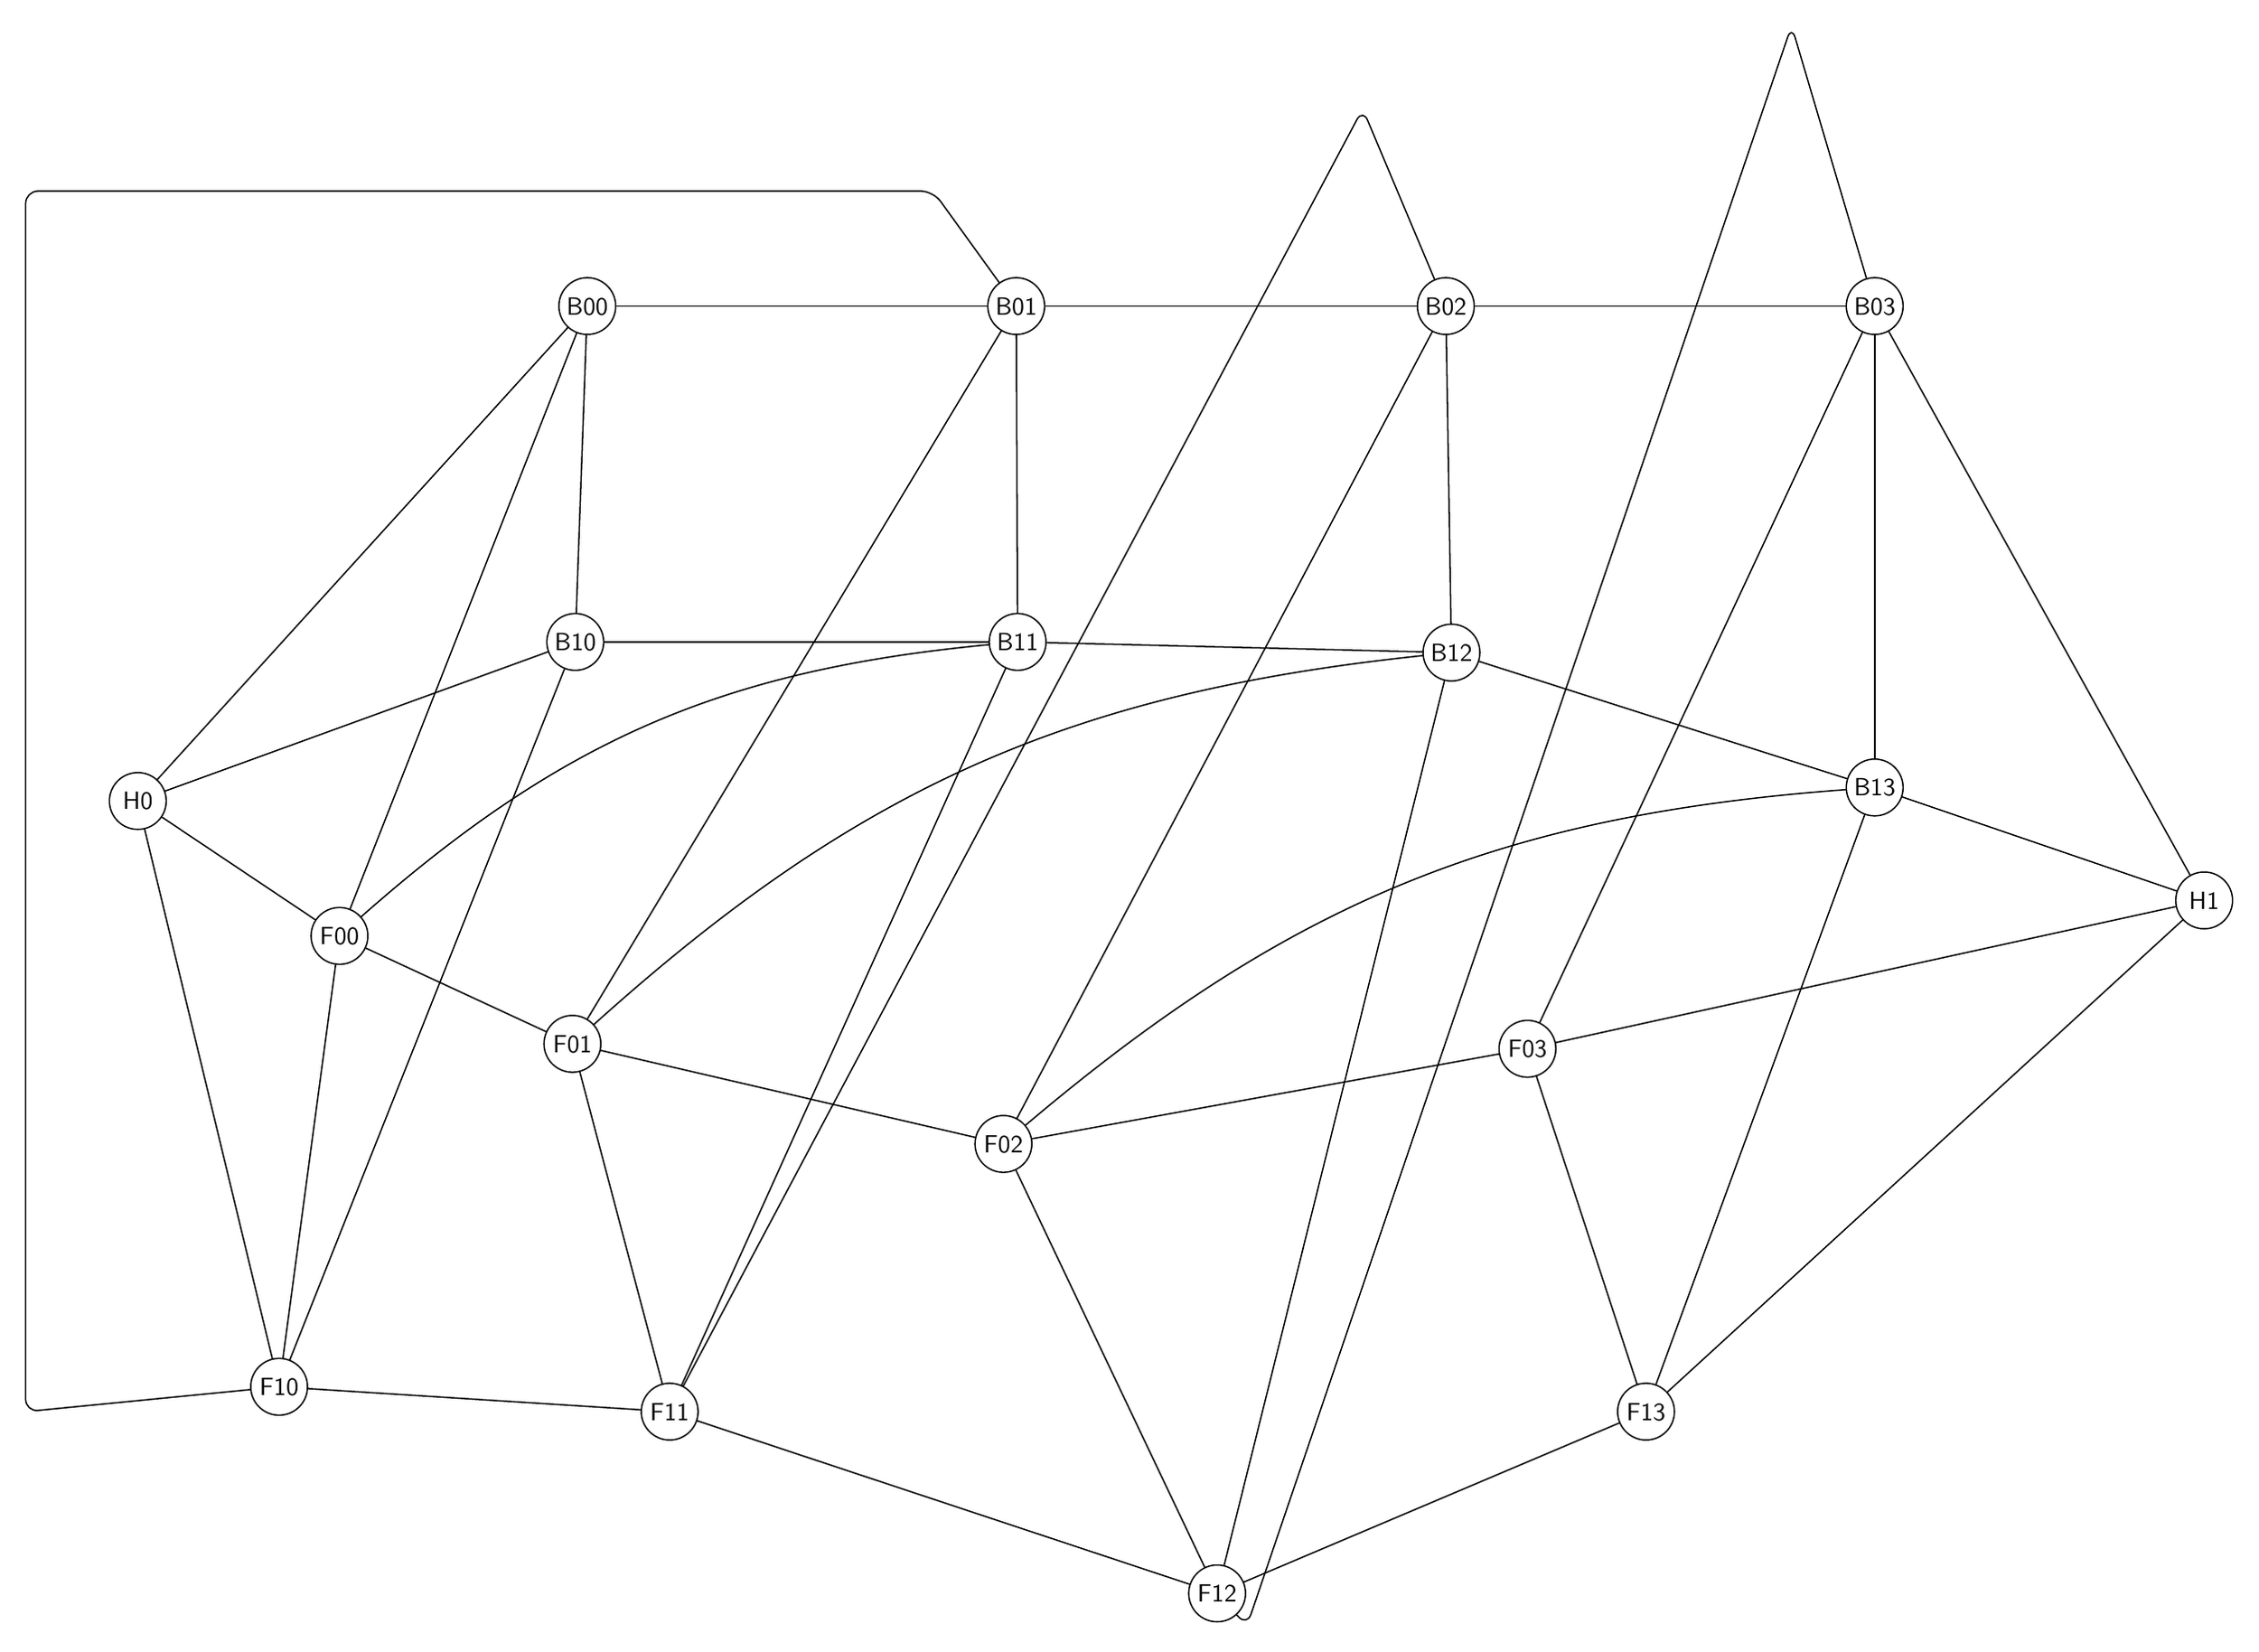
\begin{tikzpicture}[x=1cm,y=1cm]
\tikzset{
  graphnode/.style={circle,draw=black,line width=0.55pt,minimum size=8mm,inner sep=1pt,font=\sffamily},
  graphedge/.style={draw=black,line width=0.55pt,line cap=round,line join=round},
  directed/.style={graphedge,-{Stealth[length=2.4mm,width=2.0mm]}},
  undirected/.style={graphedge}
}
\node[graphnode] (n_F00) at (-10.74,0.14) {F00};
\node[graphnode] (n_F01) at (-7.46,-1.38) {F01};
\node[graphnode] (n_F02) at (-1.39,-2.79) {F02};
\node[graphnode] (n_F03) at (5.99,-1.45) {F03};
\node[graphnode] (n_F10) at (-11.59,-6.21) {F10};
\node[graphnode] (n_F11) at (-6.09,-6.56) {F11};
\node[graphnode] (n_F12) at (1.62,-9.12) {F12};
\node[graphnode] (n_F13) at (7.66,-6.56) {F13};
\node[graphnode] (n_B00) at (-7.25,9.01) {B00};
\node[graphnode] (n_B01) at (-1.21,9.01) {B01};
\node[graphnode] (n_B02) at (4.84,9.01) {B02};
\node[graphnode] (n_B03) at (10.88,9.01) {B03};
\node[graphnode] (n_B10) at (-7.42,4.28) {B10};
\node[graphnode] (n_B11) at (-1.19,4.28) {B11};
\node[graphnode] (n_B12) at (4.92,4.13) {B12};
\node[graphnode] (n_B13) at (10.88,2.23) {B13};
\node[graphnode] (n_H0) at (-13.58,2.04) {H0};
\node[graphnode] (n_H1) at (15.52,0.64) {H1};
\draw[undirected] (n_F00) -- (n_F01);
\draw[undirected] (n_F01) -- (n_F02);
\draw[undirected] (n_F02) -- (n_F03);
\draw[undirected] (n_F10) -- (n_F11);
\draw[undirected] (n_F11) -- (n_F12);
\draw[undirected] (n_F12) -- (n_F13);
\draw[undirected] (n_F00) -- (n_F10);
\draw[undirected] (n_F01) -- (n_F11);
\draw[undirected] (n_F02) -- (n_F12);
\draw[undirected] (n_F03) -- (n_F13);
\draw[undirected] (n_B00) -- (n_B01);
\draw[undirected] (n_B01) -- (n_B02);
\draw[undirected] (n_B02) -- (n_B03);
\draw[undirected] (n_B10) -- (n_B11);
\draw[undirected] (n_B11) -- (n_B12);
\draw[undirected] (n_B12) -- (n_B13);
\draw[undirected] (n_B00) -- (n_B10);
\draw[undirected] (n_B01) -- (n_B11);
\draw[undirected] (n_B02) -- (n_B12);
\draw[undirected] (n_B03) -- (n_B13);
\draw[undirected] (n_F00) -- (n_B00);
\draw[undirected] (n_F01) -- (n_B01);
\draw[undirected] (n_F02) -- (n_B02);
\draw[undirected] (n_F03) -- (n_B03);
\draw[undirected] (n_F10) -- (n_B10);
\draw[undirected] (n_F11) -- (n_B11);
\draw[undirected] (n_F12) -- (n_B12);
\draw[undirected] (n_F13) -- (n_B13);
\draw[undirected] (n_F00) to[bend left=18] (n_B11);
\draw[undirected] (n_F01) to[bend left=18] (n_B12);
\draw[undirected] (n_F02) to[bend left=18] (n_B13);
\draw[undirected,rounded corners=5pt] (n_F10) -- (-15.16,-6.56) -- (-15.16,10.63) -- (-2.38,10.63) -- (n_B01);
\draw[undirected,rounded corners=5pt] (n_F11) -- (3.67,11.79) -- (n_B02);
\draw[undirected,rounded corners=5pt] (n_F12) -- (2.04,-9.58) -- (9.71,12.96) -- (n_B03);
\draw[undirected] (n_H0) -- (n_F00);
\draw[undirected] (n_H0) -- (n_F10);
\draw[undirected] (n_H0) -- (n_B00);
\draw[undirected] (n_H0) -- (n_B10);
\draw[undirected] (n_H1) -- (n_F03);
\draw[undirected] (n_H1) -- (n_F13);
\draw[undirected] (n_H1) -- (n_B03);
\draw[undirected] (n_H1) -- (n_B13);
\end{tikzpicture}
\end{document}
